%%%%%%%%%%%%%%%%%%%%%%%%%%%%%%%%%%%%%%
% LaTeX poster template
% Created by Nathaniel Johnston
% August 2009
% http://www.nathanieljohnston.com/2009/08/latex-poster-template/
%%%%%%%%%%%%%%%%%%%%%%%%%%%%%%%%%%%%%%

\documentclass[final]{beamer}
%\usepackage[scale=1.24]{beamerposter}
\usepackage[size=a1,scale=1.1]{beamerposter}
\usepackage{graphicx}			% allows us to import images

\usepackage{subfigure}

%-----------------------------------------------------------
% Define the column width and poster size
% To set effective sepwid, onecolwid and twocolwid values, first choose how many columns you want and how much separation you want between columns
% The separation I chose is 0.024 and I want 4 columns
% Then set onecolwid to be (1-(4+1)*0.024)/4 = 0.22
% Set twocolwid to be 2*onecolwid + sepwid = 0.464
%-----------------------------------------------------------

\newlength{\sepwid}
\newlength{\onecolwid}
\newlength{\twocolwid}
\newlength{\threecolwid}
%\setlength{\paperwidth}{48in}
%\setlength{\paperheight}{36in}
\setlength{\paperwidth}{42in}
\setlength{\paperheight}{36in}
\setlength{\sepwid}{0.024\paperwidth}
%\setlength{\onecolwid}{0.22\paperwidth}  % For 4 columns
\setlength{\onecolwid}{0.30\paperwidth}   % 3 columns
\setlength{\twocolwid}{0.464\paperwidth}
\setlength{\threecolwid}{0.708\paperwidth}
\setlength{\topmargin}{-0.5in}
\usetheme{confposter}
\usepackage{exscale}

%-----------------------------------------------------------
% The next part fixes a problem with figure numbering. Thanks Nishan!
% When including a figure in your poster, be sure that the commands are typed in the following order:
% \begin{figure}
% \includegraphics[...]{...}
% \caption{...}
% \end{figure}
% That is, put the \caption after the \includegraphics
%-----------------------------------------------------------

\usecaptiontemplate{
\small
\structure{\insertcaptionname~\insertcaptionnumber:}
\insertcaption}

%-----------------------------------------------------------
% Define colours (see beamerthemeconfposter.sty to change these colour definitions)
%-----------------------------------------------------------

\setbeamercolor{block title}{fg=ngreen,bg=white}
\setbeamercolor{block body}{fg=black,bg=white}
\setbeamercolor{block alerted title}{fg=white,bg=dblue!70}
\setbeamercolor{block alerted body}{fg=black,bg=dblue!10}

%-----------------------------------------------------------
% Math commands
%-----------------------------------------------------------
\newcommand{\X}{\mathcal{X}}
\newcommand{\Y}{\mathcal{Y}}
\newcommand{\G}{\mathcal{G}}
\newcommand{\norm}[1]{\left | \left | #1 \right | \right |}
\newcommand{\reals}{\mathbb{R}}
\newcommand{\scrF}{\mathcal{F}}
\newcommand{\E}{\mathbb{E}}
\newcommand{\K}{\mathcal{K}}
\newcommand{\PP}{\mathbb{P}}
\newcommand{\N}{\mathbb{N}}
\newcommand{\Dir}{\text{Dir}}
\newcommand{\DP}{\text{DP}}
\newcommand{\Pois}{\text{Pois}}
\newcommand{\BP}{\text{BP}}
\newcommand{\BeP}{\text{BeP}}
\newcommand{\borel}{\mathcal{B}}
\newcommand{\Beta}{\text{Beta}}
\newcommand{\Discrete}{\text{Discrete}}
\newcommand{\Ber}{\text{Bernoulli}}
\newcommand{\CRP}{\text{CRP}}
\newcommand{\IBP}{\text{IBP}}
\newcommand{\Norm}{\text{N}}
\newcommand{\B}{\mathcal{B}}
\newcommand{\Corr}{\text{Corr}}
\newcommand{\Un}{\text{Un}}
\newcommand{\CRM}{\text{CRM}}
\newcommand{\NiG}{\text{NiG}}
\newcommand{\Cat}{\text{Cat}}
\newcommand{\T}{\mathcal{T}}
\newcommand{\Ga}{\text{Ga}}
\newcommand{\notrightarrow}{\centernot\rightarrow}
\newcommand{\gap}{\text{    }}



%-----------------------------------------------------------
% Name and authors of poster/paper/research
%-----------------------------------------------------------

\title{Computational statistics for whole brain CLARITY \\analysis using the Open Connectome Project}
\author{Anish K. Simhal$^1$, Will Gray Roncal$^4$, Kunal A. Lillaney$^3$, Kwame Kutten$^2$, Michael I. Miller$^2$, \\ Joshua T. Vogelstein$^2$, Randal Burns$^3$, Li Ye$^5$, Raju Tomer$^5$, Karl Deisseroth$^5$, Guillermo Sapiro$^1$}
\institute{$^1$Dept. of Electrical and Computer Engineering, Duke University  $^2$Dept. of Biomedical Engineering, Johns Hopkins University, \\ $^3$Dept. of Computer Science, Johns Hopkins University,  $^4$ Applied Physics Lab, Johns Hopkins University, \\$^5$Dept. of Bioengineering, Stanford University}

%-----------------------------------------------------------
% Start the poster itself
%-----------------------------------------------------------


\begin{document} 

\addtobeamertemplate{headline}{} 
{\begin{tikzpicture}[remember picture, overlay]
\node [anchor=north west, inner sep=3cm]  at (current page.north west)
{
\includegraphics[scale=0.5]{figs/dukelogo}};
\end{tikzpicture}

\vspace{6cm} %twiddle with this later...
\begin{tikzpicture}[remember picture, overlay]
\node [anchor=north east, inner sep=3cm]  at (current page.north east)
{
\includegraphics[scale=0.4]{figs/IID_logo}};
\end{tikzpicture}
}


\begin{frame}[t]  

\begin{columns}[t]  % align column content at top
% First column
\begin{column}{\sepwid}\end{column}  % spacer column
\begin{column}{\onecolwid} 

\begin{block}{Challenge} 

\begin{itemize}
	\item Statistically differentiate between three classes of mouse brains
\end{itemize}
\begin{figure}
	{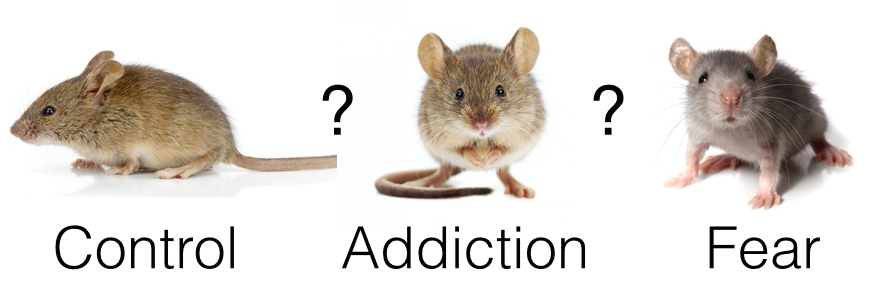
\includegraphics[scale=0.9]{figs/mouse}}
	\caption{Source: Author}
\end{figure}

\vspace{1cm}

\end{block}

\begin{block}{Background} 
The CLARITY brain clearing technique is a method for studying neurological diseases by observing structure [5]. 
\begin{figure}
	{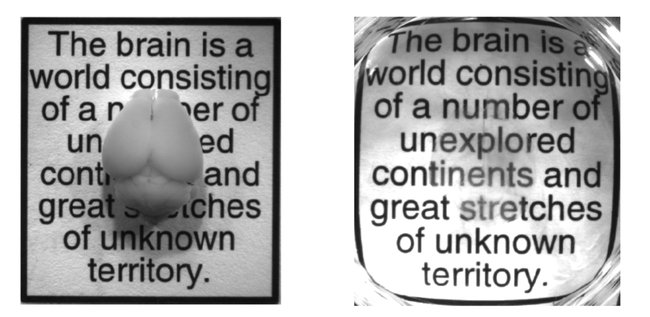
\includegraphics[scale=1]{figs/clear_clarity}}
	\caption{Effect of 'brain clearing' technique on a mouse brain. Source: New York Times}
\end{figure}

After the clearing process, each volume is imaged using light sheet microscopy. \\
\vspace{1cm}

\begin{figure}
	{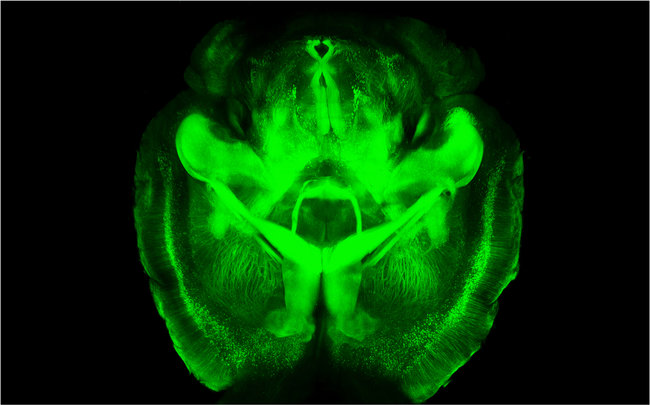
\includegraphics[scale=1]{figs/green_clarity}}
	\caption{Mouse brain imaged with light sheet microscopy. Source: New York Times}
\end{figure}
\end{block} 


\end{column}

% Second column
\begin{column}{\sepwid}\end{column}  % spacer column
\begin{column}{\onecolwid}


\begin{block}{Methods} 
\begin{itemize} 
\item{\textbf{Ingest data into the Open Connectome Project (OCP)}} 
\end{itemize} 
\begin{figure}
	{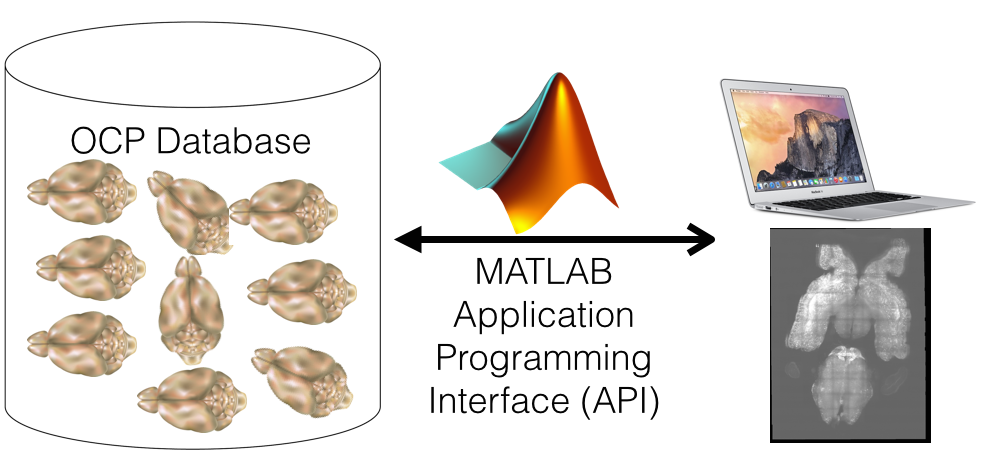
\includegraphics[scale=0.9]{figs/ocp}}
	\caption{How OCP was used in this analysis.  Source: Author}
\end{figure}
The data was hosted on servers at John Hopkins University.  Using the MATLAB API, we queried data as needed for the analysis [1].  

\vspace{1cm}

\begin{itemize} 
\item{\textbf{Register and Align to the Allen Mouse Brain Atlas}}

Each CLARITY volumes was aligned to the Allen Mouse Brain Atlas using non-linear transformations [4]. 
\begin{figure}
	{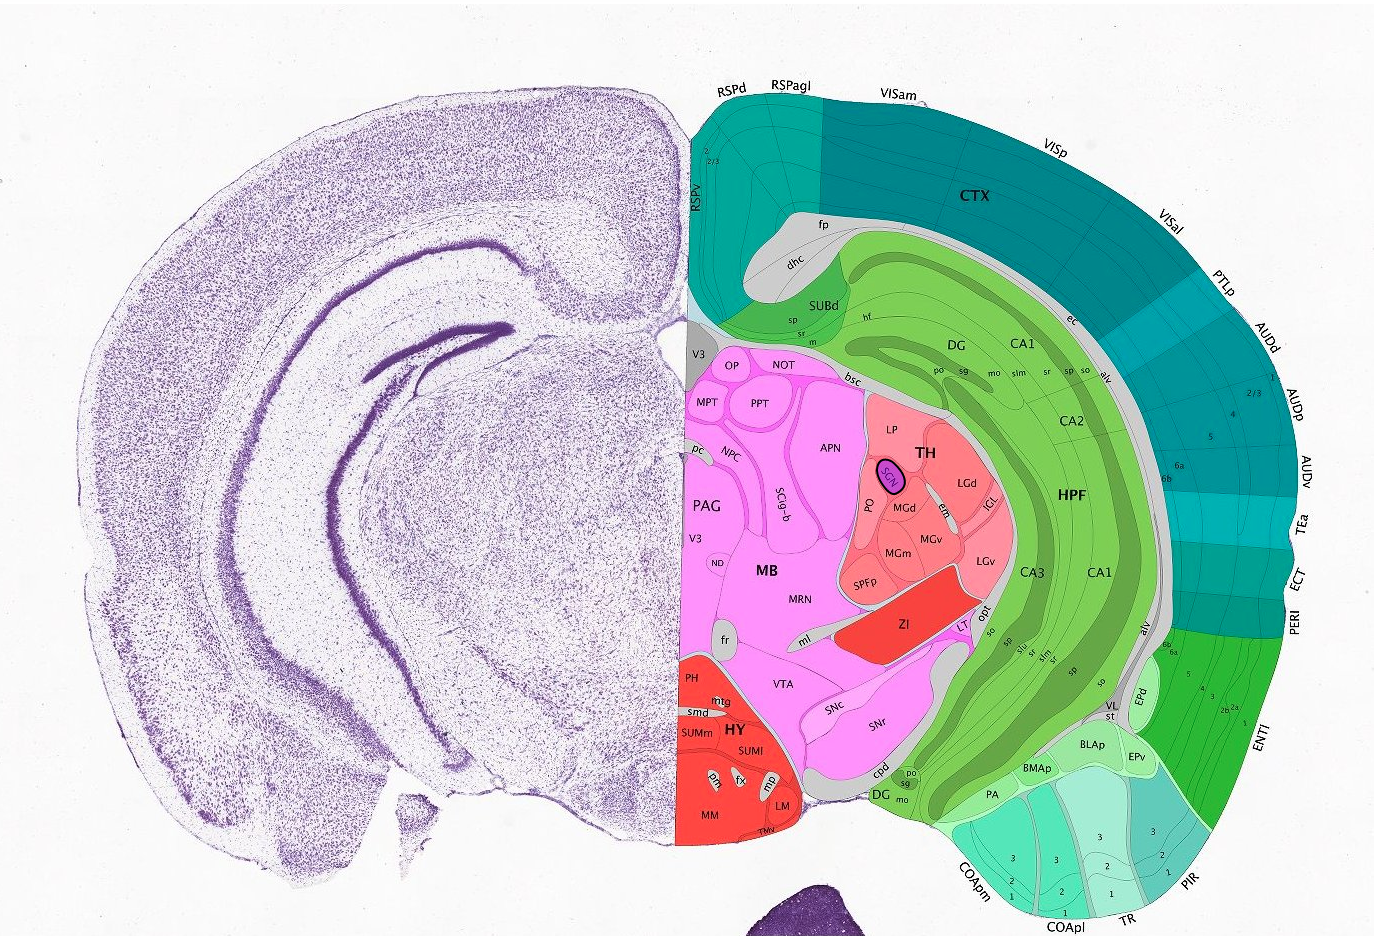
\includegraphics[scale=0.8]{figs/allenbrain}}
	\caption{Coronal slice of the mouse brain atlas, indicative of the average atlas slice.  Source: Allen Institute for Brain Science}
\end{figure}
\vspace{1cm}

\item{\textbf{Compute Haralick Features for each Region of Interest (ROI)}} 
\vspace{1cm}

For each CLARITY Volume
\begin{itemize}
	\item Normalize volume (subtract mean, divide by standard deviation) 
	\item Extract ROI 
	\item Calculate 3D Co-Occurrence Matrix and Haralick Features [3]
	\item Vectorize ROI and calculate mean, standard deviation 
\end{itemize}
Cluster and evaluate the features using the Adjusted Rand Index (ARI). 
\end{itemize}

\end{block}






\end{column}


% Third column
\begin{column}{\sepwid}\end{column}  % spacer column
\begin{column}{\onecolwid}



\begin{block}{Results} 
\begin{itemize} 
\item Demonstrated statistical differences between the various classes
\item Small number of features (1-3) are sufficient for accurate classification

\end{itemize} 

\begin{figure}
	{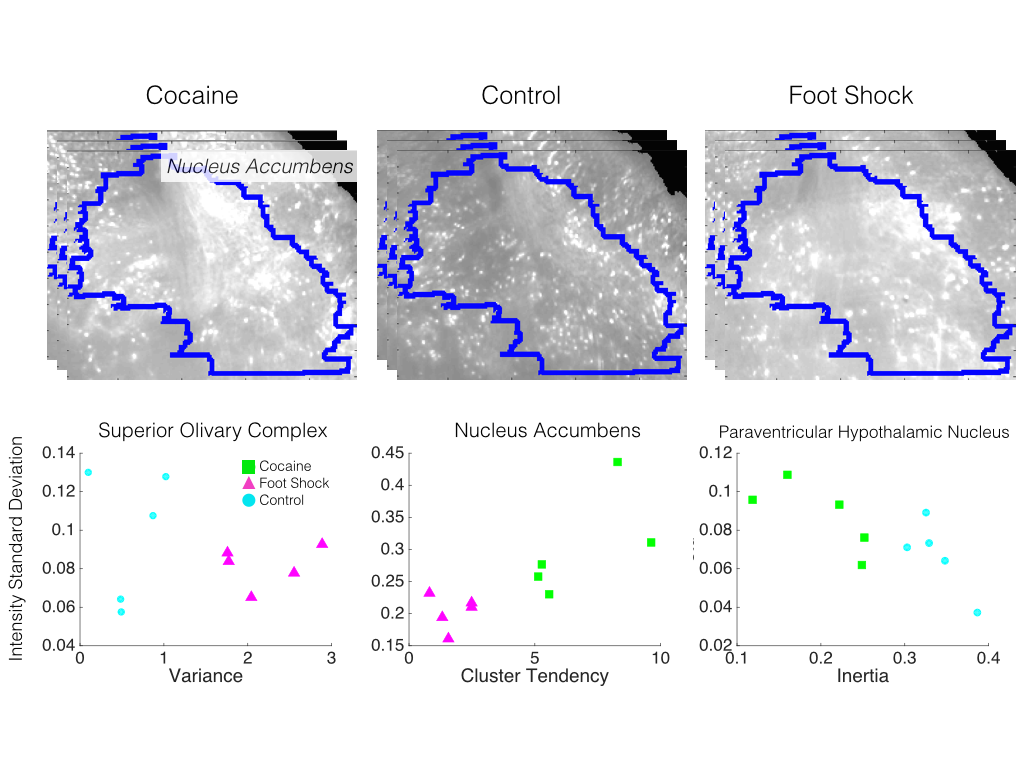
\includegraphics[scale=0.8]{figs/sfn_fig}}
	\caption{First row: Nucleus Accumbens under the 3 conditions.  Second row: three pairwise comparison plots demonstrating accurate class separation. Source: Author}
\end{figure}
\end{block} 

\begin{block}{Acknowledgments} 
\footnotesize{

This work was supported by the following grants: 
\begin{itemize} 
\item NIH NINS/NIMH 1R01NS092474 (TRA)
\item NIH 1R01DA036400 (BIGDATA)
\item NIH/NIBIB 1R01EB016411 (CRCNS)
\item DARPA N66001�14�1�4028
\item NIMH
\item DARPA NeuroFAST
\end{itemize}
}
\end{block} 


\vspace{-0.05in}
\begin{block}{References}
\footnotesize{
\begin{thebibliography}{99}
\bibitem{OCP}  Burns, R., et al. (2013). The Open Connectome Project Data Cluster: scalable analysis and vision for high-throughput neuroscience. In Proceedings of the 25th International Conference on Scientific and Statistical Database Management (p. 27). ACM.
\bibitem{nyt} Gorman, J. (2013, April 10). Brains as Clear as JellO. New York Times. Retrieved July 23, 2015, nytimes.com
\bibitem{Haralick} Haralick, R., Shanmugam, K., Dinstein, I. (1973). Textural Features for Image Classification. IEEE Transactions on Systems, Man, and Cybernetics IEEE Trans. Syst., Man, Cybern., 610-621.
\bibitem{ABA} Lein, E.S. et al. (2007) Genome-wide atlas of gene expression in the adult mouse brain, Nature 445: 168-176. doi: 10.1038/nature05453
\bibitem{CLARITY} Tomer R, Ye L, Hsueh B, Deisseroth K. Advanced CLARITY for rapid and high-resolution imaging of intact tissues. Nature Protocols. June 2014


\end{thebibliography}}
\end{block}

\end{column}
\end{columns}
\end{frame}

\end{document}
